\documentclass[11pt]{article}

\usepackage{graphicx}
\usepackage{subcaption}
\usepackage{multirow}
\usepackage{multicol}
\usepackage{adjustbox}
\usepackage{rotating}
\usepackage{amsmath}
\usepackage{float}

% \DeclarePairedDelimiter{\abs}{\lvert}{\rvert}

% \allowdisplaybreaks

\begin{document}

% \title{%
%   STAT 471/871 -- Sample Surveys and \\ Analysis of Experimental Design \\
%   \Large Assignment 2 \\
%   \large Queen's University \\
%   \normalsize Prof. Chunfang Devon Lin}

% \date{Winter, 2018}
% \author{%
% 	Filipe Roseiro Cogo\\
% 	\textit{filipe.cogo@gmail.com}}

% \maketitle

\section{growth}
\label{sec:1}

We fit a second-order model using the following equation, check the summary and analysis of variance.
\begin{verbatim}
> h<-lm(Yield~x1+x2+x3+I(x1^2)+I(x2^2)+I(x3^2)+x1*x2+x2*x3+x1*x3,data = growth)
> summary(h)
> pure.error.anova(h)
\end{verbatim}
The summay and anova table are shown as shown in figure~\ref{fig:summary_growth} and figure~\ref{fig:anova_growth}
\begin{figure}[h!]

  \center
  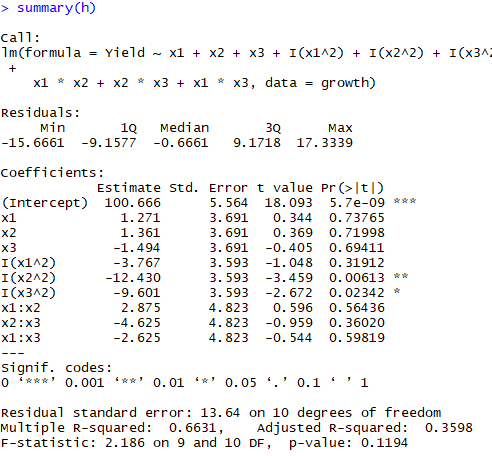
\includegraphics[scale = .45]{pictures/summary_growth.png}
  \caption{summary of second order model}
  \label{fig:summary_growth}
\end{figure}

\begin{figure}[h!]
  
  \center
  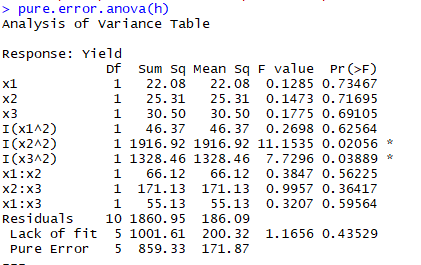
\includegraphics[scale = .45]{pictures/anova_growth.png}
  \caption{anova of second order model}
  \label{fig:anova_growth}
\end{figure}

The p-value of lack of fit is 0.43529, which is greater than 0.05. Thus, we could conclude that the second model is adequate to represent the data.
Fitted model:
$\hat{y} = 100.666 + 1.271\hat{x_1} + 1.361\hat{x_2} - 1.494\hat{x_3} - 3.767\hat{x_1}^2 - 12.430\hat{x_2}^2 - 9.601\hat{x_3}^2 + 2.875\hat{x_1}\hat{x_2} - 4.625\hat{x_2}\hat{x_3} - 2.625\hat{x_1}\hat{x_3}$
\\
$B_{3,3} = 
 \begin{pmatrix}
  -3.7670 & 1.4375 & -1.3125 \\
  1.4375 & -12.4300  & -2.3125 \\
  -1.3125 & -2.3125 & -9.6010 
 \end{pmatrix}$
,$b =
\begin{pmatrix}
   1.271\\
  1.361\\
  -1.494 
 \end{pmatrix}$
,$x_s = -\frac{1}{2}B^{-1}b = \begin{pmatrix}
    0.260\\
  0.111\\
  -0.140
 \end{pmatrix} $, and the eigenvalues of matrix B are $\begin{pmatrix}
   -3.078495\\
  -8.953226\\
  -13.766279
 \end{pmatrix} $. All eigenvalues are negative, which makes sure that $X_s$ is the maximum point.

\section{average age}
\label{sec:2}
\textbf{a)} The sample design is simple random sampling without replacement. Under SRSWOR, the sample mean $\bar{y}$ is an unbiased estimator of $\bar{Y}$, thus the estimator of mean age for children is $\bar{y} = \frac{9*13 + 10*35 + 11*44 + 12*69 + 13*36 + 14*24 + 15*7 + 16*3 + 17*2 + 18*5}{240} = 12.08$
The $v(\bar{y})$ is an unbiased estimator of $V(\bar{y})$, and $v(\bar{y}) = \frac{s^2}{n} = \frac{3.705}{240}  = 0.015$, thus, the standard error $se(\bar{y}) = \sqrt{v(\bar{y})} = 0.124$. And the 95\% confidence interval for the average age is $\bar{y} \pm Z_{\alpha/2}s\sqrt{\frac{1}{n}} = 12.08 \pm 0.243$
\textbf{b)} We determine the sample size based on this formula: $n = \frac{{Z_{\alpha/2}}^2S^2}{e^2} = \frac{1.96^2*3.705}{0.5^2} = 56.93$, hence, the minimun sample size is 57.

\section{clams}
\label{sec:3}
First, we calculate $N_h h = 1,,,4$, $N_1 = 222.81 * 25.6 = 5704, N_2 = 49.61 * 25.6 = 1270, N_3 = 50.25 * 25.6 = 1287, N_4 = 197.81 * 25.6 = 5064, N = N_1 + N_2 + N_3 + N_4 = 13325$. Then we obtain the $\bar{y_{st}} = \sum_{h=1}^{H}W_h\bar{y_h} = 1.36 $. After that, we can have the estimator of the total number of bushels $\hat{t_{st}} = N\bar{y_{st}} = 13325 * 1.36 = 18122$.

The variance of $\hat{y_{st}}$: $v(\hat{y_{st}}) = \sum_{h=1}^{H}{W_h}^2(1-n_h/N_h){s_h}^2/n_h = 0.0327$, thus, the variance of $\hat{t_{st}}$: $v(\hat{t_{st}}) = N^2v({y_{st}}) = 13325^2*0.0327 = 5806069$ the standard error is $se(\hat{t_{st}}) = \sqrt{v(\hat{t_{st}})} = 2410$

\section{totoal number of acres}
\textbf{a)}
Use ratio estimation to estimate the total number of acres:

$\hat{R} = \frac{\bar{y}}{\bar{x}} = \frac{mean(acres92)}{mean(farms87)} = 459.8975$

$\hat{t_{yr}} = \hat{R}t_{x} = 459.8975* 2087759 =  960,155,061$

\textbf{b)}
Use the regression estimation:

$\hat{\beta_0} = 263098.45, \hat{\beta_1} = 58.09$

$\hat{\bar{y}}_{req} = \hat{\beta_0} + \hat{\beta_1}\bar{x} =263098.45 +  58.09 * 2087759/3078 =   302,500$

$\hat{t}_{{yreq}} = N\hat{\bar{y}}_{req} =3078 * 302500 = 931,095,000 $

\textbf{c)}
In order to find the method with most precision, we calculate the standard variance of $ \hat{t}_y$.

ratio estimation with auxiliary variable acres87,
†
$ se(\hat{t}_{yra87}) = \sqrt{var(\hat{t}_y)} = \sqrt{N^2(1-\frac{n}{N})\frac{1}{n}\frac{1}{n-1}\sum_{i\in s}^{}{(y_i - \hat{R}x_i)^2}} = 5,344,567$

ratio estimation with auxiliary variable farms87,

$ se(\hat{t}_{yrf87}) = \sqrt{var(\hat{t}_y)} = \sqrt{N^2(1-\frac{n}{N})\frac{1}{n}\frac{1}{n-1}\sum_{i\in s}^{}{(y_i - \hat{R}x_i)^2}} = 65,364,822$

regression estimation with auxiliary variable farms87,

$ se(\hat{t}_{yregf87}) = \sqrt{var(\hat{t}_y)} = \sqrt{N^2(1-\frac{n}{N})\frac{1}{n}\frac{1}{n-1}\sum_{i\in s}^{}{(y_i - \beta_0 - \beta_1*x_i)^2}} = 58,065,813$

Based on the variances, we can tell that ratio estimation has the most precision since its variance is minimum among these three methods.

\section{Neyman allocation}
\textbf{a)}
\begin{align*} 
V_{Neyman}(\hat{t}_{str}) & = N^2V(\bar{y}_{st}) = N^2\sum_{h=1}^{H}{{W_h}^2(1-\frac{n_h}{N_h}){S_h}^2/n_h} \\ 
& = \sum_{h=1}^{H}{{N_h}^2(1-\frac{n_h}{N_h}){S_h}^2/n_h} \\
& = \sum_{h=1}^{H}{{N_h}^2(1-\frac{\frac{N_hS_hn}{\sum_{h=1}^{H}{N_lS_l}}}{N_h}){S_h}^2\frac{\sum_{h=1}^{H}{N_lS_l}}{N_hS_hn}}\\
& = \sum_{h=1}^{H}{N_hS_h(1-\frac{S_hn}{\sum_{h=1}^{H}{N_lS_l}})\frac{\sum_{h=1}^{H}{N_lS_l}}{n}}\\
& = \sum_{h=1}^{H}{N_hS_h(\frac{\sum_{h=1}^{H}{N_lS_l}}{n}-S_h)}\\
& = \frac{1}{n}\sum_{h=1}^{H}{N_lS_l}\sum_{h=1}^{H}{N_hS_h} - \sum_{h=1}^{H}{N_h{S_h}^2}\\
& = \frac{1}{n}(\sum_{h=1}^{H}{N_hS_h})^2 - \sum_{h=1}^{H}{N_h{S_h}^2}
\end{align*}

\textbf{b)}
\begin{align*} 
V_{prop}(\hat{t}_{str})  - V_{Neyman}(\hat{t}_{str}) \\
 & = \frac{N}{n}\sum_{h=1}^{H}{N_h{S_h}^2} -  \sum_{h=1}^{H}{N_h{S_h}^2} -  \frac{1}{n}(\sum_{h=1}^{H}{N_hS_h})^2 + \sum_{h=1}^{H}{N_h{S_h}^2}\\
& =  \frac{N}{n}\sum_{h=1}^{H}{N_h{S_h}^2} -  \frac{1}{n}(\sum_{h=1}^{H}{N_hS_h})^2\\
& =  \frac{N^2}{n}\sum_{h=1}^{H}{\frac{N_h}{N}{S_h}^2} - \frac{N^2}{n}(\sum_{h=1}^{H}{\frac{N_h}{N}S_h})^2\\
& =  \frac{N^2}{n}[\sum_{h=1}^{H}{\frac{N_h}{N}{S_h}^2} - (\sum_{h=1}^{H}{\frac{N_h}{N}S_h})^2]\\
& =  \frac{N^2}{n}\sum_{h=1}^{H}{\frac{N_h}{N}(S_h-\sum_{l=1}^{H}{\frac{N_l}{N}S_l})^2}
\end{align*}
\end{document}
